\chapter{绪论}

\section{分布式存储系统概述}
信息技术以及数据存储技术的发展引起了重大且深刻的社会变革,并推进了科技的进步与发展,而随着信息技术与数据存储技术在社会生活
中的不断渗入,电子数据的产生数量与速度都呈现着爆炸式的增长。根据IDC(International Data Corporation,国际数据公司)
预测,全球数据量将从2020年的44ZB增长到2025年的175ZB\cite{rydning2018digitization}。在如此急剧增长的数据体量面前,
传统的数据存储方式已然无法满足时代对于数据存储的需求,所以如何保证数据的安全存储以及便捷读取成为当前时代的一个非常重要的课题。

伴随着用户电子数据的不断增长和存储需求的不断增加,分布式存储系统凭借便捷性、统一性、安全性、可靠性得到了广泛的应用,
并且逐渐成为了当今信息社会的网络基础设施。分布式存储系统结合了负载均衡技术、集群技术、虚拟化技术、分布式技术、CDN加速技术,
为用户提供了数据存取的方便以及快捷且低成本的文件存储服务。

但是,目前流行的云存储系统普遍依赖中心服务器来提供云存储和数据处理服务\cite{wang2018blockchain}。
存储节点本身硬件故障或者技术原因导致的风险等原因会导致存储在服务器上的数据丢失或者永久不可访问。
从而导致存储的数据永久性的丢失。例如:2018年腾讯云因磁盘故障导致文件元数据的丢失,大量的个人用户资料数据丢失;\citet{sathiamoorthy2013xoring}曾
指出“Facebook数据中心的一个大集群在一个月内的节点故障数目超过20个而一天内失效节点的数量峰值可高达100个”。
因此如何提高分布式存储系统的数据可靠性亦即数据修复技术是业界和学术界广泛关注的问题。对于可靠性低且经常发生故障的海量存储节点,
如何采用性能优越的技术和措施才能保证数据的可靠性和故障发生时如何以相对低廉的成本快速修复故障节点的数据是目前研究的重要方向。

目前,分布式存储系统通常采取超过原本1倍的冗余数据来保证数据可靠性以对抗节点故障而导致的数据丢失,
进而通过冗余数据进行相关的计算还原出丢失的数据。分布式存储系统中冗余数据的产生方法大致可以分为两类:
\begin{enumerate}
	\item 多副本方式,即将数据对象复制多份(通常为三份),如$r$份,然后将这些副本均匀地分散到$r$个不同的存储节点上,
	      当某个节点故障时,只需要从剩下任意节点中下载原文件$r-1$次,并将其重新存放到其他正常节点即可。但是在数据存储急剧增长的情况下,备份冗余会引发大量存储开销,早期的分布式集群一般采用这种方式。
	      其中典型的代表有Google File System\cite{ghemawat2003google},Hadoop Distributed File System\cite{borthakur2008hdfs}等。
	\item 纠删码方式,即使用纠删码(erasure codes)技术生产冗余数据块。纠删码是通过编解码矩阵的计算创建了远小于多备份技术的冗余数据,同时提供同级别的容错性\cite{weatherspoon2002erasure}。
	      如今的大规模存储群越来越多地采用纠删码\citep{ford2010availability,huang2012erasure,muralidhar2014f4,ovsiannikov2013quantcast},进而取得存储空间和可靠性二者之间的均衡。
	      具体的编码方式则是将原始文件计算分割成若干个数据块,再进行编码生成多个冗余的编码块。与多副本方式相比,纠删码的优点在于能够极大地节省了存储空间,
	      进而减少了存储空间上的开销。目前学术界有大量的纠删码的编码方式,如Reed-Solomon码(简称RS码)\cite{reed1960polynomial},
	      Regenerating Code(简称RGC码)\cite{wu2009reducing},Local Regeneration Code(简称LRC码)\cite{kamath2014codes}等。
\end{enumerate}

无论是多副本技术还是纠删码方式都会产生冗余数据,并且都有其固有的缺陷。多副本技术消耗了更多的存储空间,
消耗$(m-1)$倍于原始数据大小的存储空间,例如三副本机制在大数据时代,
当数据规模达到PB、EB甚至ZB级别时,多副本技术极高的存储空间成本以及维护开销将使得数据中心无法承担。除此之外,纠删码自身也存在着
相应地无法忽视的缺陷,例如修复成本过高、消耗大量的CPU资源进行编解码操作、实现过程复杂等,从而使得将该技术应用到分布式存储系统中时面临着诸多挑战。

\section{数据容错技术概述}

通常采用数据容错技术来对系统的可靠性和访问性进行提升。数据容错技术是指通过对存储数据进行冗余,并将冗余数据传输到其他节点上,使得即使一部分数据失效也可以通过
其他节点将数据进行恢复。

为了保证系统中数据的快速访问,在部分数据因节点故障而丢失时必须利用健康节点上的剩余数据快速地将
数据重新恢复出来,此过程被称为“\textbf{数据修复(Data Repair)}”\cite{li2009tree}。维持数据原有
的冗余度是数据修复技术想要达到的目的,同时也要确保数据的可靠性。因为对于数据容错技术而言,能够容忍的数据
丢失是极其有限的,一旦丢失的数据超过了容错技术的容忍度,原本的数据对象将无法恢复,从而导致数据的永久性丢失。
一般的数据修复过程主要遵循以下过程:当系统检测到节点故障事件产生时,根据系统设定的容错方案开始进行启用对应的修复方案,
利用剩余的健康数据节点对丢失的数据进行恢复,通过一定的算法将数据分散存储到存活节点中去,在这个过程中修复时提供数据的节点称为提供节点,修复出的
数据存在的节点称为新生节点。分布式存储系统冗余机制可以分为结构容错机制和数据容错机制。

\subsection{结构容错机制}
结构容错机制实现系统容错的方式是通过提供冗余的物理设备的方法来实现的。具体的分类方式是根据冗余物理设备的
不同可以分为以下两种:基于节点冗余的冗余机制和基于链路冗余的容错机制。

基于节点冗余的容错机制实现文件冗余的方式是使用增加冗余节点的方式实现的。当系统中的某个数据节点失效以后,
系统将使用冗余节点替代失效节点\cite{ghemawat2003google,hua2009smartstore,weil2004dynamic}。

基于链路冗余的容错机制则是通过增加冗余的网络链路的方式来实现文件冗余。主要通过两种方式进行实现,其中之一为
通过在树结构的上层链路加入冗余链路来提高系统容错性\cite{al2008scalable,greenberg2011vl2},
或者通过在服务节点上添加网卡的方式实现多链路冗余\cite{guo2008dcell,guo2009bcube}。

\subsection{数据容错机制}
在传统的分布式存储系统中,用户节点通过将文件切块后再将数据块分发到存储节点中。通过创建冗余的数据编码块来
对分布式存储系统的容错能力进行提高的方式被称为数据容错机制。根据冗余数据编码块创建方式的不同,数据容错
机制可以分为基于复制的容错机制和基于编码的容错机制。
\begin{figure}[htbp]
	\centering
	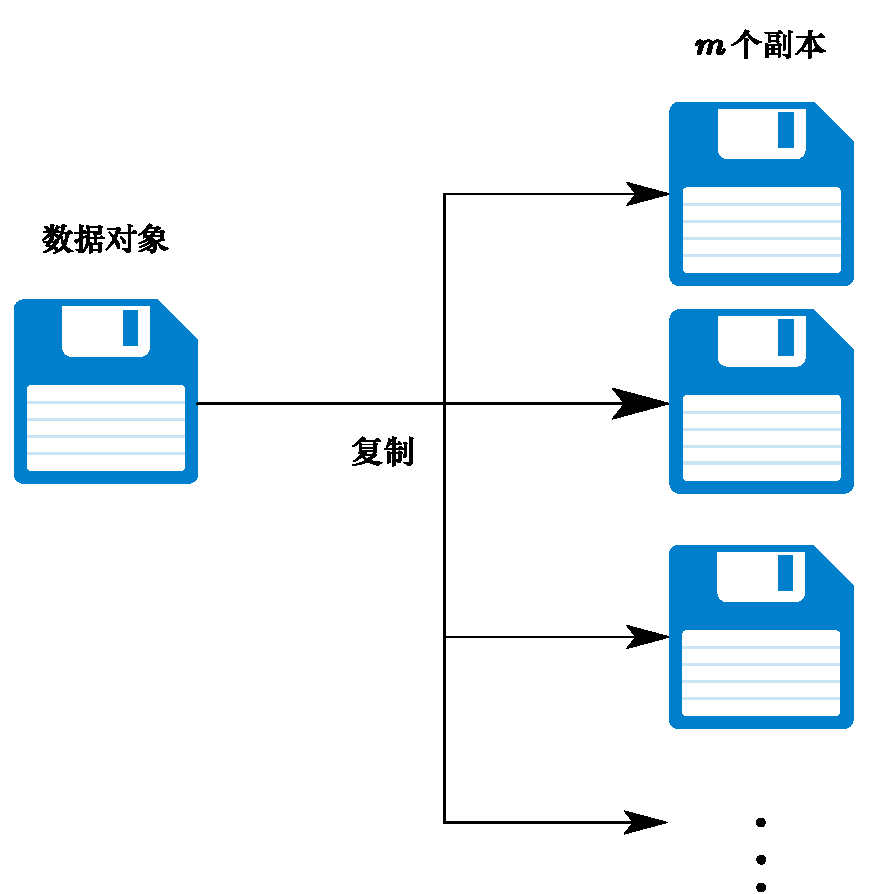
\includegraphics [scale=0.5]{figures/1.1.pdf}
	\caption{基于复制的容错机制原理}
	\label{fig:con-1.1}
\end{figure}

基于复制的容错机制原理如图~\ref{fig:con-1.1}所示,将原始数据复制多份,创建多个数据副本并分发到不同的存储节点上
从而实现数据冗余\cite{shvachko2010hadoop,ghemawat2003google,王意洁2017分布式存储中的纠删码容错技术研究}。
当一个或者多个存储着原始文件副本数据的存储节点故障时,系统通过访问其他存活节点的原始文件的副本数据,进行数据的恢复,
进而提高系统的可靠性。基于复制的冗余机制原理较为简单,易于部署和实现,并且在确保数据可靠性的基础上还能提高数据的并发访问能力。
然而,缺点显而易见,在文件储存过程中,需要分发多个多个数据副本,因此提高了数据的存储开销和通信数据的开销,存储效率较低。
对于$n$副本的复制容错机制,系统存储空间的总体利用率只有$\frac{1}{n}$。在此基础之上,为了提高存储效率,降低存储空间的开销,
可以采用动态复制机制,依据系统的网络状况、用户需求等因素进行综合考量并进行动态创建与删除副本\cite{lakshman2010cassandra,gill2016dynamic,gai2012design}。
但是,动态复制技术也存在其固有的缺陷,因为在动态创建与删除副本的过程中,需要CPU执行大量的计算,并且需要进行频繁的数据分发,从而
增加了系统的计算开销和通信开销。


相对应的,基于编码的容错机制首先对原始数据文件进行切块,再对切成的块文件进行编码,
生成体积较小的编码块从而提高数据可用性。
基于编码的容错机制生成的编码块体积小、数量少,因此,相对于基于复制的容
错机制,具有较小的存储开销。基于编码的容错机制可以分为两种:RAID技术、纠删码容错。

RAID技术\cite{patterson1988case,chen1994raid}是一种传统的基于编码的容错技术,RAID技术实现容错的方式
是通过将数据进行条带化,然后将数据条带分发到不同的存储节点上,并生成一个编码块进而实现数据的容错与冗余。
RAID技术一般只能容忍一到两个数据块的失效,因此对于大规模的分布式存储系统而言,RAID技术无法满足其数据可靠性的要求。

更加主流的基于编码的容错方式便是纠删码技术,其本身是一种编码容错技术,最早被应用到通信领域,解决数据
在传输中的纠错问题。传统的纠删码技术实现容错机制的步骤一般如下,首先将原始数据文件分割成$k$个数据块,
然后将这些数据块通过相应的矩阵计算进行编码生成$n-k$个编码块,最后将生成的$k$个数据块和$n-k$个编码块分发到
不同的存储节点中。当用户访问存储系统下载数据时,只需要从$n$个数据块中任意下载$k$个可用的块即可恢复出完整的
原始数据文件。

相较于基于复制的容错技术即多副本技术,纠删码技术的优势主要体现在更加低的存储成本同时提供更加稳定的数据修复方式\cite{lin2004erasure,weatherspoon2002erasure}。
例如,RS(12, 10)码可以凭借0.2倍的额外存储空间开销
获取两个节点的容错能力,这比具有同等容错能力的三副本技术节省了约60\%的存储空间。在同等的存储空间利用的情况下,
以纠删码技术构建的分布式系统的数据可靠性比采用多副本技术构建的分布式存储系统中的数据可靠性要大几个数
量级\cite{lin2004erasure,weatherspoon2002erasure}。
尽管有很多代表性的工作\citep{huang2019lower,xu1999x,reed1960polynomial,roth1989mds}对于纠删码的计算性能进行了优化,
但是纠删码方案由于其固有的缺陷如大量的矩阵计算编解码操作,依然会产生巨大的通信开销。因此如何提高纠删码容错的效率是一个亟需解决的重要问题。

\section{纠删码概述}
近年来,越来越多的大规模存储系统采用了具有较强容错能力和空间利用率较高的纠删码实现系统冗余\citep{xia2007robustore,kubiatowicz2000oceanstore}。
随着时代发展,数据规模越来越大,如何提升纠删码的容错能力用以满足系统的存储和访问需求已然成为学界与业界广泛关注的问题。

纠删码的主要思想是把一个数据对象$D$分为$k$个相同大小的数据块,运用异或计算和矩阵计算从而生成
$n$个块($n>k$),使得通过其中任意$k'$个块即可重新还原出原始数据,具体过程如图~\ref{fig:con-1.2}所示。

\begin{figure}[htbp]
	\centering
	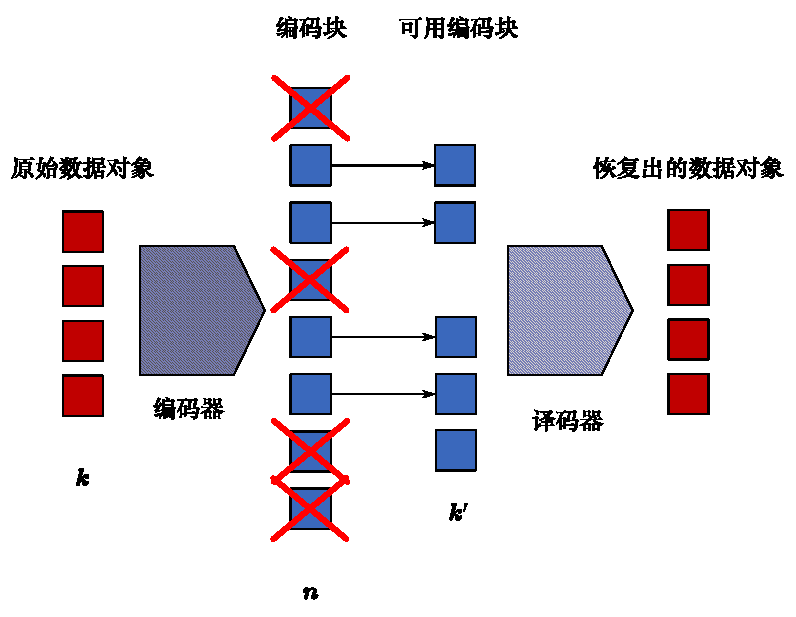
\includegraphics [scale=0.8]{figures/1.2.pdf}
	\caption{纠删码编码和解码示意图}
	\label{fig:con-1.2}
\end{figure}



一般来说,纠删码的通用表示方法为$(n,k,k')$。其中$k$是对象切分成的块数,$k'$是一个不小于$k$的数,
$n$是编码后的块数。首先,将$D$分割成$k$个大小(平均)相等的数据块$D_1,D_2,...,D_k$,然后通过数学算法和
矩阵运算将这$k$个数据块进行编码,生成$n$个同等大小的编码块$I_1,I_2,...,T_n,n>k$,使得
通过其中任意$k'$个块都能通过矩阵运算还原出$D$的对应的$k$个数据块$D_1,D_2,...,D_k$,从而组合出原始的数据。
纠删码可以容忍的最多失效块的个数称为容错度,当$k=k'$时,纠删码达到理论上的最高容错力,称之为最大距离可分码
(Maximum Distance Separable,简称MDS码)\cite{blaum1996mds}。这样的纠删码通常可以表示为
$(n,k)$,如果纠删码生成的$n$个块集合中包含全部的$k$个原数据块,这样的纠删码便是系统码(System Code)\cite{plank2009raid}。
对于系统码而言,编码后生成的额外$n-k$个块称为编码块,并且记为$P_1,P_2,...,P_m$,其中
$m=n-k$,系统码可提升系统性能,这也是现有的纠删码大多是系统码的原因。

在存储系统实际的运行过程中,先将文件分割成固定大小的数据块,进而将这些块每$k$个作为一组,每组
独立进行编码操作生成$n$个块,其中$n$个块的集合称为一个条带(Stripe)\cite{hafner2005matrix},
$k$称为条带长度(Stripe Length)。
当数据对象的块数不能被$k$的整除时,则对相应的数据域以0填充,被0填充的部分只是在逻辑上存储在磁盘中,
在数据修复时也不需要读取。根据计算方式和几何构造的不同,纠删码可分为Reed-Solomon码、阵列结构型纠删码、
网络编码型纠删码和分组结构型纠删码。

\subsection{Reed-Solomon码}
Reed-Solomon码\cite{reed1960polynomial}是最为经典的MDS码,是唯一可以用任意的数据磁盘数目和任意冗余磁盘
数目的MDS码。RS码的编码原理是通过矩阵的运算来完成的,如果分布式存储集群采用的是结构为
$(k+r,r)$的RS编码,则整个分布式存储集群应具有$k$个数据块和$r$个编码块。
在基于RS编码的分布式存储集群中,如图~\ref{fig:con-1.3}所示,编码块是通过将$k$个数据块
与$k\times (k+r)$个生成矩阵相乘来构造的,该生成矩阵主要包含了两个变量,一个
$k \times k$校验矩阵和一个$k \times r$冗余矩阵\cite{li2016procode}。一个由$(k+r,r)$
组成的RS编码存储集群,含有$k+r$个存储节点的阵列,其中$k$个数据块和$r$个编码块分别存储在存储集群中的
$k$数据节点服务器和$r$个奇偶校验节点服务器上。

\begin{figure}[htbp]
	\centering
	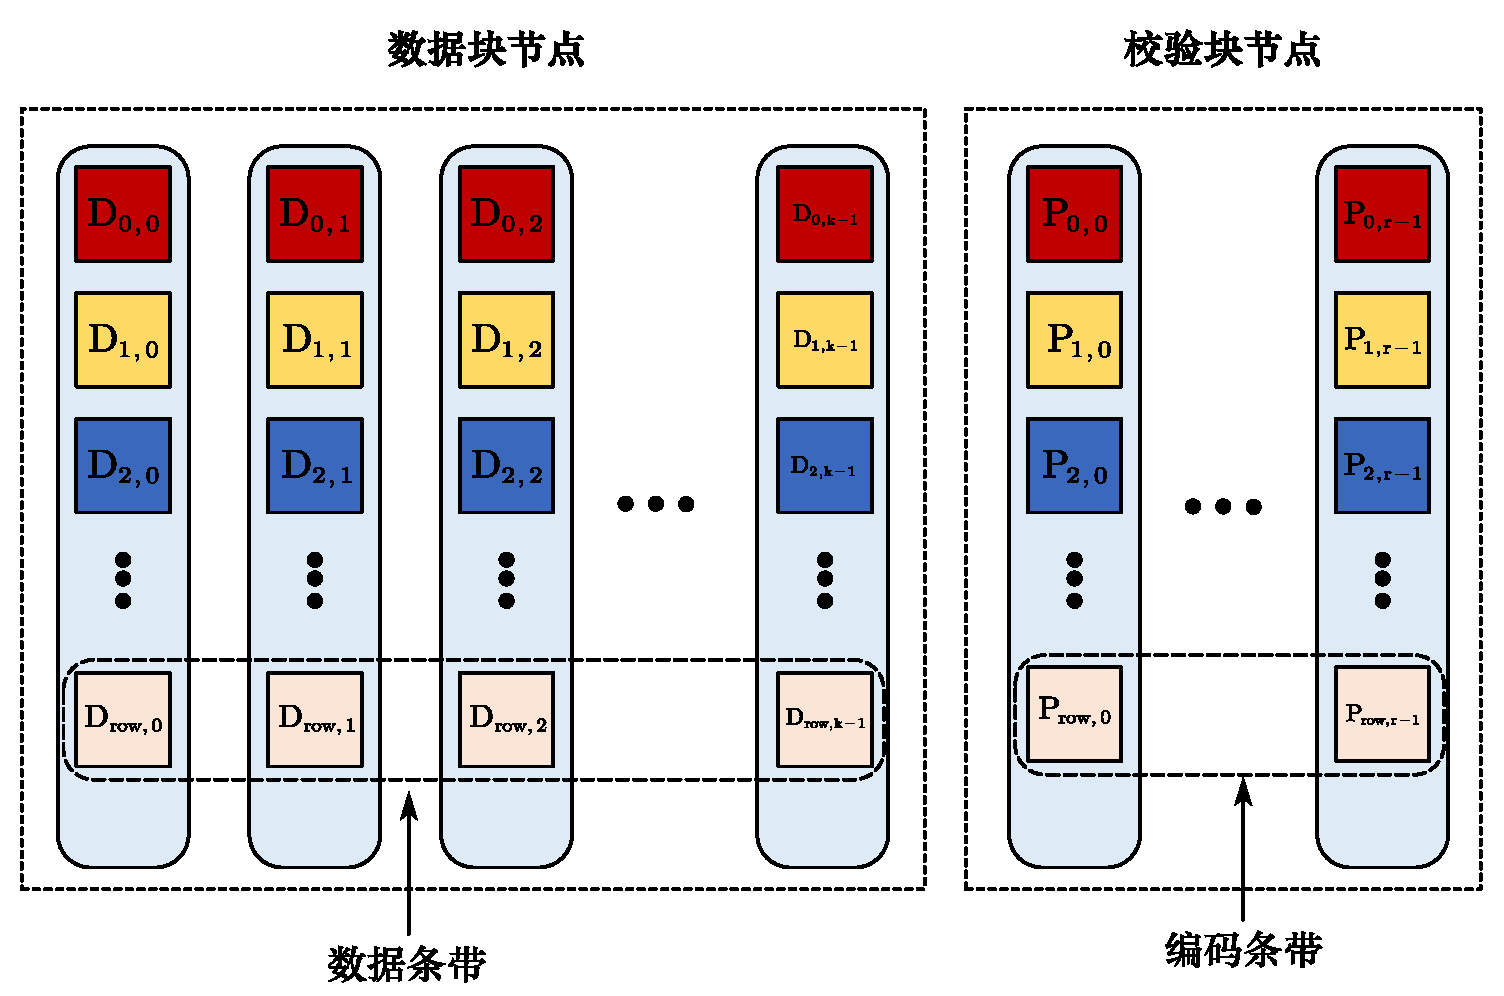
\includegraphics [scale=0.5]{figures/1.3.pdf}
	\caption{传统基于RS码结构的存储集群布局}
	\label{fig:con-1.3}
\end{figure}

RS码实际上是利用生成矩阵和数据列向量进行矩阵乘法得到编码列向量。
RS码
使用的生成矩阵$G$中的任意$k$行组成的矩阵需要在Galois域上可逆,故获得生成矩阵的计算量并不低,且可由范德蒙德(Vandermonde)矩阵或柯西(Cauchy)矩阵\cite{roth1989mds}通过变换得到。
通过相应的方法计算得到的RS码分别称为范德蒙德RS码和柯西RS码。在Galois域上,异或运算被定义为加法,
使用离散对数运算和查表来进行乘法运算,因此计算开销很大,而应用柯西矩阵可将乘法运算转化为二进制
的乘法运算,从而减轻运算量。

% RS码拥有比传统多副本容错更高的容错能力和更高的灵活性。RS码不仅达到了理论上的最高
% 容错能力,而且其条带长度$k$可以取任何大于0的整数,编码后产生块数$n$可以
% 取任何大于$k$的整数。$n$相对于$k$越大,RS码的容错能力越高,但存储空间消耗
% 也越多。因此,RS码在可靠性和存储空间开销方面给予了系统很大的选择空间。
然而,纠删码的其中一个弊端在于会引起大量的带宽以及计算资源的消耗,进而导致存储效率的降低。
大量的矩阵计算所产生的计算开销增加了系统的修复开销,
使其在分布式存储系统中的应用有很多亟待解决的问题。
与此同时,RS码可以提供优秀的容错能力以及更加低的空间消耗,从而对提高分布式存储系统的数据可靠性和降
低其经济成本具有重大意义。为了解决这一问题,涌现出了众多修复成本较低的纠
删码。这些低修复成本的纠删码根据其采用的基本技术可以分为三类:基于阵列结构的纠删码
、基于网络编码的纠删码和基于分组结构的纠删码。

\subsection{基于阵列结构的纠删码}
阵列码是一种采用阵列结构编码且完全基于异或运算的纠删码,从
冗余磁盘阵列(RAID)\cite{patterson1988case}技术中不断发展出来。
其主要思想就是将数据块和校验块存储到二维矩阵内,根据其放置方式的不同,可以分为横式阵列码和纵式阵列码。

横式阵列码(horizontal parity array codes)的特点是将数据块和校验块分别传输到不同的存储节点上。
在这样的系统中专设有冗余磁盘来存储冗余数据,正常的数据块存储在正常的磁盘中,从而提高阵列码的可扩展性。


EVENODD编码\cite{blaum1995evenodd}是最早被发表的阵列码,EVENODD码的编码块和数据块之间的计算关系
如图~\ref{fig:con-1.4}所示。其中第一列上的编码块分别由各自同一行上的其他数据块进行异或得到。此外,RDP\cite{corbett2004row}编码也是
一种应用较为广泛的横式阵列码,这些编码体系均对磁盘数目提出了严格的要求(要求磁盘数目必须是素数或者素数减1),
同时还要求在单个条带中的数据元素的个数必须与磁盘的数目相匹配。

除了EVENODD和RDP,其他的横式阵列码有EEO\cite{feng2010eeo},
STAR\cite{huang2008star},
RAID-6 Liberation\cite{plank2009raid}和Feng's Code\cite{feng2005new}等,
它们具有性能比较优秀的编码效率和极高的存储空间利用率。由于横式阵列码本身固有的缺陷,如写入数据总会用到冗余磁盘,
故其中的I/O流量成为了横式阵列码的性能瓶颈。


\begin{figure}[htbp]
	\centering
	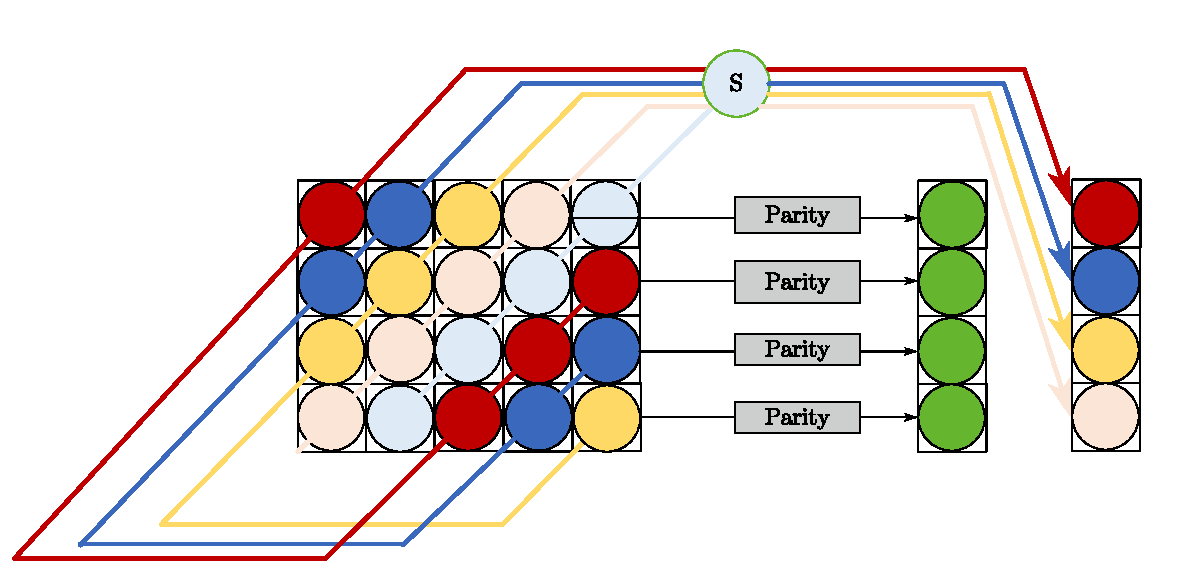
\includegraphics [scale=0.7]{figures/1.4.pdf}
	\caption{EVENODD码的编码结构示意图}
	\label{fig:con-1.4}
\end{figure}

纵式阵列码(vertical parity array codes)是指冗余存储在数据条带中的阵列编码方式,
将数据块和校验块不加区分地存放节点的磁盘中。这样的方式会将计算操作和写入操作平均地分摊到各个磁盘上,实现了负载均衡。
X-code\cite{xu1999x}是具有MDS性质的纵式纠删码,其在编码操作,数据更新以及数据重构等步骤上具有
理论上的最优效率,缺点就是可扩展性比较差。


X-code的编码方法如图~\ref{fig:con-1.5}所示,
每一列的元素存储在同一个数据节点中,
每个节点上存储着$k$个编码块。其中红色块代表数据块,蓝色块代表编码块,$n$需要是一个大于2的素数,数据个数必须
为$n-2$个,编码块的个数也必须是2个。此外,第一个编码块由主对角线上的数据块进行计算得到,另外一个编码块由副对角线
的数据块计算得到,这些计算需要用到$k$个磁盘上的数据块,计算成本较高,且修复时需要按照一定的顺序进行计算,失去了并行
修复的可能,这些均是X-code的不足之处。

\begin{figure}[htbp]
	\centering
	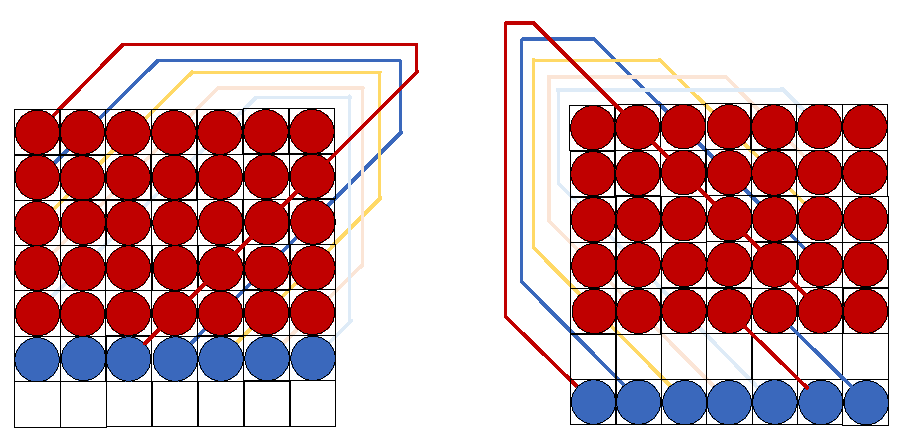
\includegraphics [scale=0.7]{figures/1.5.pdf}
	\caption{X-code的编码结构示意图}
	\label{fig:con-1.5}
\end{figure}


阵列码在计算上的主要特点就是所有的运算都是异或运算,相较于传统的RS编码在计算性能上有优化,但需要的数据量却并没有
丝毫减少,传输的数据量较大。


\subsection{基于网络编码的纠删码}
网络编码最初由\citet{ahlswede2000network}于2000年首次提出。
网络编码优化了网络中节点的功能,使得其不仅可以
存储转发数据,并且还可以在转发数据之前对数据进行编码和矩阵计算,从而
提高了网络吞吐率。

\citet{dimakis2010network}将网络编码的思想应用到纠删码上并称之为再生码
(Regenerating Codes)。
再生码允许新生节点访问多于$k$个节点,从而显著降低修复过程需要传输的总数据
量。


\begin{figure}[htbp]
	\centering
	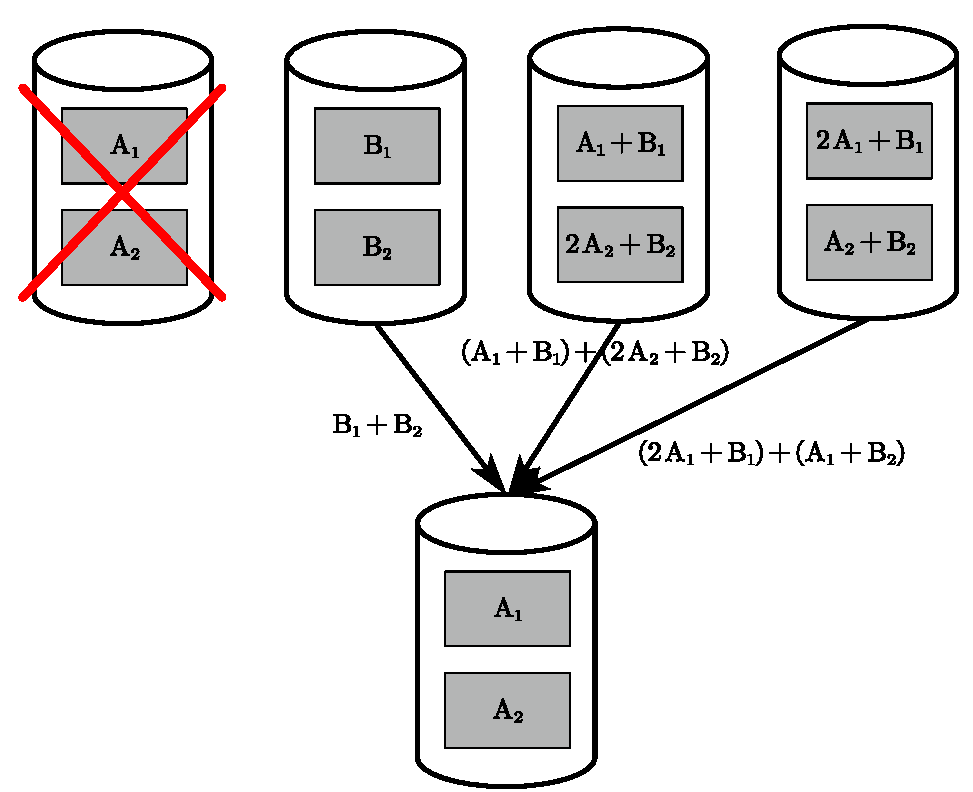
\includegraphics [scale=0.6]{figures/1.6.pdf}
	\caption{再生码修复失效数据节点示意图}
	\label{fig:con-1.6}
\end{figure}

图~\ref{fig:con-1.6}显示了再生码修复失效数据节点过程,总共有四个用来存储数据的节点,
并且每个存储
节点上存放着两个数据块,并且是通过相关的矩阵运算生成的。
再生码修复数据的方法是首先在存储节点中进行计算后再进行数据分发,
传输数据块的总数目为3,相较于传统的修复方法,再生码修复数据传输量降低
了25\%。


\citet{dimakis2010network}提出的再生码可以对丢失的数据进行精确修复,
但对编码块只能进行功能性修复。
这里修复出的数据并不等同于原来的数据但是可以与原来的存储系统维持相同的容错度。
针对此问题,
\citet{wu2007deterministic}提出了确定性再生码
(Deterministic Regenerating Codes),并从概率学角度证明了其存在性。

根据存储效率的不同,再生码可以分为$\frac{k}{n}\leqslant \frac{1}{2}$的低比特率码和
$\frac{k}{n}> \frac{1}{2}$的高比特率码。一般来说,这样的方式可以减少数据的传输量,
但是由于编码系数所在域的要求限制、选择方法的不规则和难以实现等原因,目前应用并不广泛。


\subsection{基于分组结构的纠删码}
基于分组结构的纠删码可以减少数据修复时需要下载的数据量,因传统的RS码在修复一个丢失的块时
需要下载的数据条带长度为$k$,而分组结构的纠删码的方法则是将$k$减小从而达到降低数据量的目标。
分组编码的纠删码首先将数据条带分成若干组,各个组各自计算相应的编码块,实现组内修复丢失块,需要的块数
则取决于每个组内的数据块数。
RS码其实是一种特殊的分组编码,可以看成将整个数据条带作为一组,此外根据
分组方法的不同,此类纠删码可以分为两类:水平分组结构的纠删码和交叉分组结构的纠删码。

比较经典的水平分组纠删码一般是将数据条带分为两组。每个小组生成一个局部的冗余块,然后整个条带
再生产一个全局的冗余块。这样数据修复就可以依靠小组内的编码块完成,降低了修复成本。图~\ref{fig:con-1.7}显示的是微软的
Azure系统\cite{calder2011windows}采用LRC(Local Reconstruction Codes)\cite{huang2012erasure}
的一个实际的例子LRC(8,2,2)。可以看出,它将数据块平均分为了两组,每组各自内部计算出一块局部冗余编码块,
相当于一个RS(5,4)码。对于两个条带再生成2个全局的校验块,则相当于一个RS(10,8)码。当丢失块数不多时,例如丢失1个块,则只需要4个块即可进行数据修复,
这样就有效降低了修复成本。



由此可以发现,组数越多,那么可以容忍的失效的块数也就越多,故Pyramid码\cite{huang2013pyramid}便诞生了,
它的特点就是可以对条带内的数据块进行任意层次的分组,层次越多平均的修复成本也就越低,但是相对的存储空间消耗也就越大,
因为产生了更多的全局校验块,对于Pyramid码需要根据实际的存储系统环境选择更加适中的方案。除此以外水平结构
的编码还有运行在Facebook旗下的分布式存储系统中的XORing Elephants\cite{sathiamoorthy2013xoring}、
EXPyramid\cite{周松2011expyramid}、LRCs\cite{sathiamoorthy2013xoring}等。EXPyramid码是对两层
Pyramid码的一种改进,其分为了三组。


\begin{figure}[htbp]
	\centering
	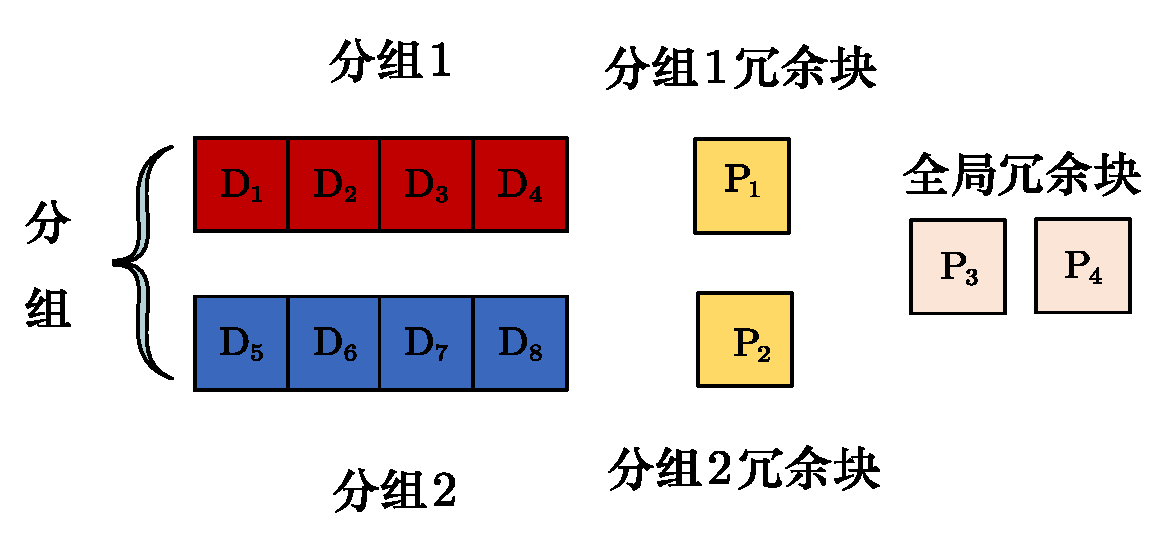
\includegraphics [scale=0.5]{figures/1.7.pdf}
	\caption{LRC(8, 2, 2)的编码示意图}
	\label{fig:con-1.7}
\end{figure}


交叉分组结构的纠删码与水平分组不同之处大致有两点。第一,交叉分组纠删码的分组方式不同,交叉分组
的各组之间相互重叠但却互不包含,相比之下水平分组各组之间一般不重叠且会有一个全局的校验块包含着各个分组的校验块。
第二,交叉分组纠删码编码计算较为简单,基于异或计算。不难看出,交叉分组有着相对来说较低的计算性能消耗的优点。常见的交叉结构的
纠删码有\citet{woitaszek2007tornado}提出的Tornado码,如图~\ref{fig:con-1.8}所示,其任何组别的冗余块均为组内的数据块的校验块,并且
修复任何一个数据块或者冗余块只需4个或3个块,避免了大量下载编码块的特殊情况。此外还有
LDPC\cite{gallager1962low}、WEAVER码\cite{hafner2005weaver}和Tanner码、Hover码\cite{hafner2006hover}等。

\begin{figure}[htbp]
	\centering
	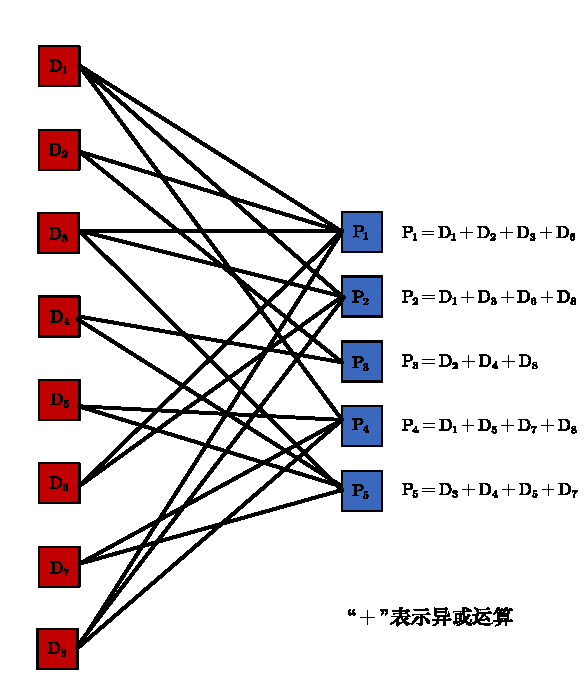
\includegraphics [scale=0.8]{figures/1.8.pdf}
	\caption{Tornado码的构造示意图}
	\label{fig:con-1.8}
\end{figure}

\section{基于纠删码的数据修复技术}
在基于纠删码的分布式存储系统中,数据传输并不是简单的线性路线,每当修复一个数据块时,
提供者节点要向新生节点传输若干数据块从而进行计算,数据的传输路径往往比较多样化,根据传输
路径的不同一般可分为两种修复技术:基于星型拓扑的数据修复、基于树型拓扑的数据修复。除此之外,还有一种基于XOR的纠删码数据修复技术。

\subsection{基于星型拓扑的数据修复}
基于星型拓扑的串行修复技术(Star Structure Based,SSR)是按照顺序修复最近失效的数据块,修复过程遵循星型结构。
\citet{dimakis2010network,wu2007deterministic}提出的再生码数据修复过程要求每个存活节点向
新生节点传输均等的数据量进行修复,数据收集节点(DC节点)仅连接$k$个节点,通常
是$k-1$个数据节点和第一个校验数据节点,并从每个节点下载$\frac{M}{k}$的数据量($M$为原文件大小)。这里存在一个
非常明显的缺陷,节点可以选择的链路比较单一,带宽较高的链路很有可能会被忽视,导致修复效率降低。
\citet{shah2010flexible}提出了弹性修复的方法,即允许存活节点和DC节点充分利用所有可用的链路,
从中选择带宽较大的链路进行数据传输,传输的数据不均等。DC节点驱动任务从节点$i(1 \leqslant i \leqslant n)$
获取$\mu_i (0 \leqslant \mu_i \leqslant \alpha)$,其中需要满足总的获取量不小于$M$即可。同理,新生节点从存活节点
$i(1 \leqslant i \leqslant n)$接收$\beta_i (0 \leqslant \beta_i \leqslant \beta_{max})$
数据量,满足总接收量大于或等于一个设定参数$\gamma$即可,用不等式表示
则如式~\ref{eq:1-1}和~\ref{eq:1-2}:

\begin{equation}
	\label{eq:1-1}
	\sum_{i=1}^{n} \mu_{i} \geq M, 0 \leq \mu_{i} \leq \alpha
\end{equation}
\begin{equation}
	\label{eq:1-2}
	\sum_{i=1}^{n} \beta_{i} \geq \gamma, 0 \leq \beta_{i} \leq \alpha
\end{equation}

节点发生故障时,新生节点可以确定从任意$k$个节点下载$\frac{M}{k}$的数据量,修复产生的流量相等于原文件大小。
对于弹性修复方法而言,新生节点,可以根据可用带宽的大小从不同节点上下载不均等的数据来降低修复时间。
当然星型拓扑的缺点也很明显,DC节点需要收集多个节点的数据,修复速度会受到磁盘和网络I/O的限制,编解码的计算消耗也很大。

\subsection{基于树型修复拓扑的数据修复}
上节所描述的星型拓扑的技术其实是树型拓扑修复技术的特殊情况,然而修复速度受到了诸多的制约,为了提升修复的速度,
树型拓扑修复方法因此被提出。

\citet{li2009tree,li2010tree}独辟蹊径地首次设计了一个新的基于网络带宽的树形修复方法(Tree-structured Data Regeneration),
利用木桶原理并通过提高最低传输速度来加速数据的修复。
修复路径与树结构类似,组成的元素包括提供者节点和新生节点。提供节点主要是接收数据和对数据进行存储和计算然后再进行转发,在这过程中
生成树结构,其中最大生成树是最优的修复树。


树型修复方法是对星型修复方法的改进,传统的方法在修复时每个节点承担的修复任务繁重,导致
节点在I/O性能和计算上很难取得一个良好的平衡,有大量节点处于闲置状态,这样整个系统的资源就没有完全利用起来。
树型修复方法利用树结构的优势可以将计算任务和传输任务在网络中并行地进行,同时可以利用流水线优化技术,加速修复任务的进行。
当然缺点也比较明显,在网络带宽变化较快的环境中,树型修复的带宽判断往往不是当前网络的最优,容易陷入局部最优,而在全局来看也同样浪费了部分资源。

另外两类比较经典的树型修复修复技术分别是根据网络拓扑优化的NTar\cite{许方亮2013ntar}和面向
多节点修复的并行修复技术\cite{weidong2013tree}。NTar提出了网络距离的概念,综合考量传输流量和网络距离来加速修复。
并行修复技术\cite{weidong2013tree}构建了分离边策略和共享边策略,目标是充分地利用网络资源,其存在的问题也比较明显,
即会出现无法建立树型路径的可能以及空闲带宽没有完全得到充分利用。

\subsection{基于XOR的纠删码数据修复}



\citet{xiang2010optimal}提出的基于异或运算(XOR)的纠删码低网络负载数据修复技术
,专门用于优化RDP码\cite{corbett2004row}
修复失效数据所传输的数据量。
\citet{khan2012rethinking}将其理论进行一般化并拓展到异或运算上,任何通过异或运算构建的纠删码都可以采用这种修复方式。
目前有三种比较主流的基于异或运算的纠删码数据修复方
法,根据修复目标的不同,可以分为三种方法,分别面向优化降级读性能的方法、降低修复时间的方法以及降低修复成本的方法。

面向优化降级读性能的方法。降级读主要针对的是数据的暂时失效,即在请求读取系统数据时,先将数据构建出来进行读取,然后再进行修复操作。
对于带宽不对等问题,
\citet{zhu2014boosting}提出了枚举贪心算法(Enumerated Greedy Algorithm),简称
EG算法,EG算法通过排列组合计算出$d$个可用节点可能的情况,确定在每一种组合下有$l$个CDREs,并且为每个CDREs计算其降级读时间,更新
降级读时间,使每个块的降级读时间最小。

降低修复时间的方法。\citet{niu2013phr}针对RAID-6编码系统提出了多条带修复的策略,其将修复过程划分为三个部分,同时还考虑了系统I/O和节点的带宽不对等性,
提出了并行不对等修复算法(parallel heterogeneous recovery),简称
PHR算法。算法对三个部分的修复过程分别进行了优化,并且是按顺序执行的,各个条带修复呈现相对独立,通过线程技术和流水线修复技术可以加速修复任务,从而降低修复时间。

降低修复成本的方法。针对同一条传输路径上由于带宽不对等造成的成本差异,\citet{zhu2012cost}结合传输成本和带宽性能
,定义修复总成本为$\mathrm{C}=\sum_{i=0, i \neq k}^{p} w_{i} y_{i}$,,其中假设节点$k$失效,$w_i$表示从节点$i$读取一个
对象的成本,$y_i$表示从节点$i$读取的对象数目,进而他们提出了基于传输成本的异构恢复(cost-based heterogeneous recovery)算法,简称CHR算法。
CHR算法所有的最小读取量恢复序列进行枚举,并且计算这些序列的修复成本的总和,返回其中最小的总修复成本对应的修复序列。


% \section{纠删码及修复技术的问题和挑战}

\section{论文主要研究内容}
本文面向纠删码存储系统中的数据预先修复问题和混合纠删码问题,以纠删码技术为基础,以高可靠性、低存储成本和高修复速度为目标,
对纠删码数据修复速度低,修复代价高等问题开展研究。

(1)预先数据修复技术研究

纠删码面临的最基本问题就是过量的修复开销:修复流量随着存储冗余度的降低
而增加。因此,前人对改善纠删码的修复性能进行了广泛的研究,使修复过程中的
修复流量或I/O最小化,或设计适用
于所有实践中的纠删码包括RS码的提高修复效率的技术。目前,大部分的传统修复方法都
是被动修复,只有在检测到节点故障后才会触发修复操作。如果可以提前预测即将发
生的故障,就可以在任何实际故障发生之前主动修复任何即将发生的节点故障,以提
高系统可靠性。

针对反应式修复降低系统可靠性问题,通过结合迁移与重建来设计实现预先修复的机制,用以修复STF(Soon To
Fail)节点。对于重建集与迁移集问题,设计了划分迁移集与重建集算法
SMSRS(Split Migration Set And Reconstruction Set)算法,根据中继节点的特性,提出了 ISA(Improved SMFRepair Algorithm)算法来
进行节点修复的调度,使得反应式修复慢的问题得到了缓解和优化。

(2)混合纠删码数据修复技术研究

在传统的存储系统中大多只采用一种纠删码进行
数据的处理和存储,这种方式一般先将文件分割成固
定大小的数据块,再将这些数据块每$k$
个作为一组,
每组独立进行编码操作生成$n$
个块,其中$n$
个块的集合
称为一个条带(Stripe),然而这种方式难以在保持低
存储空间消耗的情况下降低退化读的延迟时间。

针对单一纠删码的延迟问题,在前人工作的基础上,提出了一种可感知数据热度的负载动态自适应
的混合纠删码(LRC\&HH)数据修复方案。旨在根据真实储存系统数据修复场景中
的数据 I/O 的特点,以及数据访问和故障事件的时空局部性,提出更加符合相应情况
的混合纠删码修复方案,从而对于计算开销型修复任务降低其开销和存储成本,对读
取密集型和频繁重建型修复任务降低其工作负载,并加速系统的修复速度和减少重
建时间。


(3)基于混合纠删码的容错存储原型系统设计与实现

为了进一步验证本文的理论研究成果,本文设计实现了基于混合纠删码的容错存储原型系统。
该系统有三个特点:1)基于开源分布式存储中心
的离散事件模拟器 SimEDC 进行设计实现;2)含有丰富的混合纠删码方案,包括
已有的 HACFS、EC-Fusion以及LRC\&HH,支持相应的扩展接口;3)支
持修复调度中的重建与迁移的融合。容错存储原型系统设计主要包含以下模块:存储中心架构,节点故障模型,混合
纠删码策略,节点放置策略,可靠性度量指标,事件处理模式。实验结果表明,基于混合纠删码结构的容错存储原型系统具有较高的可靠性,
PDL、NOMDL和BR都有一定程度的降低,系统可靠性得到提升。


\section{论文组织结构}

本文共分为六章,研究方向技术路线如图~\ref{archi}所示,各章节组织结构如下:

第一章:绪论。论述了课题的研究背景和意义。介绍了分布式存储系
统和分布式存储系统中的数据容错问题;概述了纠删码技术及基于纠删码的数据修复技术,简述了本文的主要研究内容。

第二章:相关研究。综述了与本文主要工作相关的研究内容,主要包括编码结构优化的数据修复技术、调度优化的数据修复技术、带宽优化的数据修复技术、
基于混合纠删码的数据修复技术和基于预先修复的数据修复技术等并总结了
各种技术的优点与不足。 

第三章:基于预先重建迁移的数据修复技术研究。首先介绍了预先修复的重建技术和迁移技术的修复细节;然后提出了重建和迁移集的划分算法,结合
中继节点的概念提出了预先修复的调度算法;最后通过对比仿真实验评估了预先修复算法的性能。

第四章:基于混合纠删码的数据修复技术研究。首先分析了混合纠删码的编码策略选择方案LRC和HH码;对自适应策略的编码分配进行了
数学分析与验证并提出自适应选择算法;然后分析了与自适应策略相对应的编码切换算法,并进行了算法分析;最后通过数据集的仿真实验,
对自适应策略与传统方法进行了对比分析比较。

第五章:基于混合纠删码的容错存储原型系统设计与实现。介绍了本文设计实现的混合纠删码容错存储系统,包括总体架构、数据修复的基本流程
以及混合纠删码的实现方式,并通过仿真实验对系统的可靠性进行了分析。

第六章:总结与展望。总结本文的主要研究工作并指出未来的研究方向。

\begin{figure}[H]
	\centering
	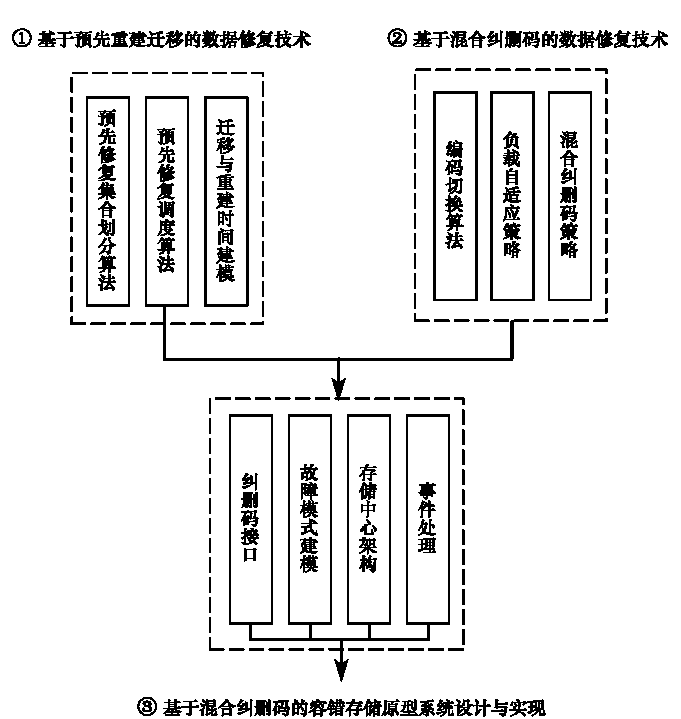
\includegraphics [scale=0.95]{figures/archi.pdf}
	\caption{本文研究点技术路线}
	\label{archi}
\end{figure}


